\chapter{Comprensión de Programas}

\section{Introducción}

La \textit{Comprensión de Programas} es una disciplina de la Ingeniería de Software
cuyo objetivo es proveer \textit{Modelos, Métodos, Técnicas} y \textit{Herramientas}
para facilitar el estudio y entendimiento de los sistemas de software \cite{BeronHenriquesPereira10}.

La importancia de la Comprensión de Programas radica en que es una de las demandas cognitivas
más importantes, dentro del conjunto necesario para llevar adelante las tareas implicadas
en el proceso de desarrollo y sus distintas fases \cite{PetreDeQuincey06}.
La correcta aplicación de los modelos, métodos, técnicas y herramientas propuestas por
la Comprensión de Programas, hacen que el desarrollador pueda localizar y entender rápidamente
los elementos empleados para soportar una funcionalidad específica, disminuyendo el tiempo requerido
para la realización de una tarea, impactando positivamente en los costos asociados a la
modificación, mantenimiento y evolución de un sistema \cite{BeronHenriquesPereira10}.

La forma que tienen los programadores de entender un sistema, componente o pieza de código fuente
puede ser descrita a través de diferentes modelos, los cuales componen la base para las herramientas
de comprensión de programas \cite{BeronHenriquesPereiraUzal07}.
Éstos son denominados \textit{modelos cognitivos}.
La información necesaria para aplicar los modelos cognitivos, se obtiene a través de
\textit{métodos de extracción de la información}.
Para facilitar la compresión y el proceso establecido en el modelo cognitivo, se utilizan
diferentes técnicas de \textit{visualización de software}, y así procesar mejor la
información extradía por distintos métodos.
Por último, diferentes \textit{estrategias para la inter-conexión de dominios} pueden ser
aplicadas para que el programador asocie el dominio del problema, con el dominio
del programa bajo estudio.

Las siguientes secciones, desarrollan sobre los conceptos nombrados previamente.

\section{Modelos de Comprensión de Programas}

Generalmente se establece que la \textit{comprensión}, dentro de este ámbito de estudio, es un
proceso en el que el individuo construye su propia representación mental de un programa.
Si bien existen varias escuelas de pensamiento, independientemente de las diferencias, la
mayoría de los modelos de comprensión de programas contiene un conjunto común de elementos,
tal como se puede ver en la Figura X \cite{SchulteClear10}.

\begin{figure}[H]
    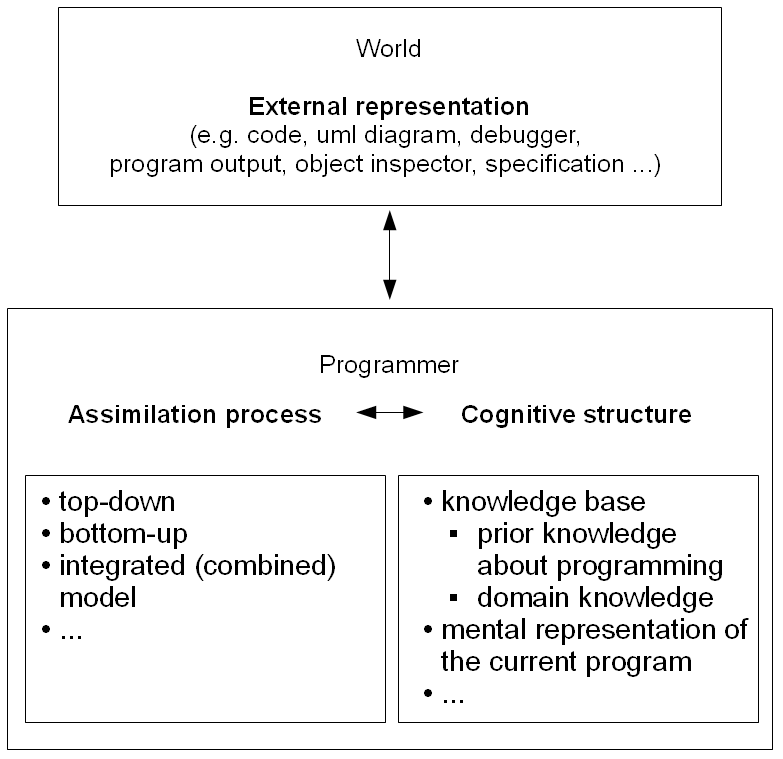
\includegraphics[width=10cm]{program_comprehension/elements.png}
    \centering
    \caption{Elementos principales de los modelos de comprensión de programas}
\end{figure}

\subsection{Representación Externa}
Se considera que la representación externa son todos aquellos materiales asociados al programa
en estudio que el programador puede utilizar para su proceso de comprensión, pero que no son 
parte del conocimiento interno del individuo.
Estos elementos pueden ser presentados de diversa forma, incluyendo directamente el código fuente,
hasta manuales, documentación, diagramas UML, entre otros.

\subsection{Estructura Cognitiva}
El conocimiento interno de un programador, el cual puede dividirse entre base de conocimiento
y representación mental, es lo que se define como estructura cognitiva.

La base de conocimiento viene dada por el conocimiento general que el programador posee,
independiente de la aplicación específica que se está tratando de comprender.
Esto incluye conocimiento general de lenguajes y principios de programación, algoritmos, 
aplicaciones similares y demás.

El modelo mental es una representación interna al programador del software bajo consideración.
Determina el nivel de conocimiento del individuo sobre el sistema en cuestión, y es construido
a medida que se comprende, utilizando la base de conocimiento mencionada anteriormente.
Diferentes elementos, tanto estáticos como dinámicos, forman parte del modelo y permiten
su evolución.\cite{MayrhauserVans95}

\subsection{Proceso de Asimilación}
La estrategia implementada por los desarrolladores para extraer información de un programa, 
construir una representación mental del mismo, y así lograr su comprensión, es lo que se
conoce como proceso de asimilación.

\begin{description}
    \item[Top-down] Los modelos de comprensión top-down son aquellos que implican la
    aplicación de conocimiento sobre el dominio del programa y la correlación de este
    conocimiento con el código fuente del mismo.
    En el modelo de Brooks, una sucesión de hipótesis forma el proceso de asimilación.
    En el esquema de Soloway y Erlich, los programadores utilizan planes y reglas de programación
    para descomponer objetivos y planes en otros planes de menor abstracción.
     
    \item[Bottom-up] Caen dentro de esta clasificación aquellos modelos en
    los que su proceso de asimilación comienza con las sentencias de código fuente, y
    las mismas se van agrupando y así obteniendo mayores niveles de abstracción.
    El proceso se repite una y otra vez, hasta lograr una representación mental completa
    del programa en cuestión.
    En el proceso de asimilación propuesto por Pennington, se presentan dos modelos diferentes.
    El modelo del programa, que se obtiene de agrupar microestructuras en macroestructuras, y
    se corresponde con una abstracción del flujo de control del programa.
    El modelo de situación, incluye el flujo de datos dentro del programa, y representa la
    función y objetivos del mismo.
    En el modelo de Shneiderman y Mayer, la base de conocimiento se compone tanto de
    conocimiento sintáctico como semántico.
    A mayor experiencia del desarrollar, mayor será este último.

    \item[Oportunista] Algunos autores consideran que, dependiendo
    de la necesidad de comprensión para la tarea en cuestión, no existe un enfoque
    sistemático de resolución.
    Algunos autores consideran que no existe un enfoque sistemático de asimilación,
    y que dependiendo de la necesidad de comprensión, un programador puede aprovechar
    las estrategias tanto bottom-up como top-down.
    Letovsky plantea que un programador puede procesar la información de forma bottom-up
    o top-down a medida que van apareciendo pistas que ayuden a su comprensión.
    
    \item[Modelos Integrados] Los modelos integrados suponen una combinación de los
    anteriores, en donde el proceso de asimilación implica ir cambiando de
    modelos a medida que se requiera, para poder construirlos simultáneamente.
    Se plantean tres representaciones mentales: el modelo del dominio, el modelo del
    programa y el modelo de situación.
    Es muy importante la base de conocimiento del programador, ya que le va a permitir
    la construcción de las representaciones.

\end{description}

\section{Métodos de Extracción de la Información}

Para poder lograr comprender una pieza de código fuente o programa bajo estudio, un
programador debe ser capaz de poder obtener información del mismo.
El tipo de información que el usuario necesita, depende de la tarea que tenga que llevar
adelante respecto al software.
Dentro la disciplina de Comprensión de Programas, para extraer la información requerida 
por los diferentes procesos cognitivos, se utilizan dos tipos de análisis de código:
\textit{Análisis Estático} y \textit{Análisis Dinámico}.

El \textbf{análisis estático} del software consiste en obtener información sobre el 
sistema de interés, pero sin ejecutarlo.
Los \textit{analizadores sintácticos} operan a nivel de código fuente, empleando
técnicas tanto de \textit{pattern matching} como de construcción de árboles de sintáxis
abstracta (\textit{Abstract-Syntax Tree}).
Los \textit{analizadores semánticos} trajaban de una manera diferente, ya que consideran
la secuencia en la que pueden darse los estados de un programa, en una ejecución.
La premisa principal consiste en que analizar los posibles estados de un programa en un
punto determinado, son suficientes para probar propiedades estáticas del mismo.
\cite{Cousot77}

El \textbf{análisis dinámico} corresponde a la extracción de propiedades de un sistema
en ejecución.
Estas propiedades son obtenidas al examinar una o más ejecuciones de un programa, a
través de diferentes técnicas.
Generalmente, se obtiene a través de la instrumentación del código fuente, y así
analizar los aspectos que son de interés; y es muy dependiente del input que reciba
el programa.
\cite{Ball99}

\section{Visualización de Software}

La visualización de software refiere al uso de diversos elementos (texto, 
gráficos 2D y 3D, diagramas, imágenes, vídeos, entre otros) para representar algún
aspecto de un programa y facilitar su comprensión.\cite{PetreDeQuincey06,Chen06,GomezHenriquez01}
Estos aspectos u objetos de interés pueden ser abstracciones de componentes, de
un sistema completo e incluso del comportamiento en tiempo en ejecución de los
mismos. \cite{TeysereCampo09}

Las visualizaciones pueden ayudan al programador con tres procesos cognitivos
\cite{ButlerAlmond93}:
durante un proceso de descubrimiento o exploratorio, en donde el usuario no
sabe específicamente qué está buscando;
durante un proceso de toma de decisión o analítico, en el cuál el usuario sabe lo que
está buscando y sólo necesito encontrarlo;
durante un proceso descriptivo, en el cuál es conocido el patrón que aparece en los
datos pero necesita una visualización acorde para expresarlo.

Estos procesos cognitivos que se pueden ver beneficiados por las visualizaciones, suelen
emplearse en diferentes tareas que puede llevar a cabo un programador.
Dentro de esta lista de tareas \cite{MalleticMarcusCollard02} encontramos: desarollo,
debugging, pruebas, mantenimiento y detección de errores, re-ingeniería, ingeniería reversa,
administración del proceso de software, y marketing.
En las primeras etapas del desarrollo de un nuevo sistema o aplicación, las visualizaciones
permiten la colaboración entre desarrolladores y ayudar en la definición y validación de los
requerimientos.
A medida que se avanza en la construcción del software, las herramientas permiten validar
los avances y encontrar defectos.
En el caso de mantenimiento, ayudan en la comprensión del programa, entender su diseño y
así plantear su evolución \cite{PetreDeQuincey06}.

Algoritmos, programas y sistemas son los diferentes alcances que se consideran
dento de la disciplina de Visualización de Software.\cite{PriceBaeckerSmall93,Myers90}
La Visualización de Sistemas se emplea para representar el sistema en su conjunto,
a través de los diferentes módulos que lo componen.
En la visualización de Programas, se busca mostrar el comportamiento de los mismos
y la relación entre sus componentes \cite{BenAri01}.
Por último, la Visualización de Algoritmos se utiliza principalmente en el campo de la enseñanza,
para demostrar el funcionamiento de algoritmos y estructuras de datos.
Así mismo, tal como denota la expresión 
"Alg. V isualization < P rog. V isualization < Sys. V isualization"\cite{BeronHenriquesPereiraUzal07}
las técnicas implementadas en un determinado alcance, pueden ser implementadas
también en un conjunto de mayor nivel de abstracción.

La taxonomía de Price, Baecker y Small \cite{PriceBaeckerSmall93}, establece que
existen seis categorías de atributos para los sistemas de visualización.
Dentro de las mismas podemos encontrar:
\begin{enumerate}
    \item \textbf{Alcance:} refiere al espectro de programas que pueden ser analizados.
    \item \textbf{Contenido:} corresponde al conjunto de propiedades del sistema que se pueden
    extraer y visualizar.
    \item \textbf{Forma:} relacionada a la salida de los resultados de la visualización.
    \item \textbf{Método:} determina cómo está especificada la visualización.
    \item \textbf{Interacción:} referida la manera en la que el usuario pueda controlar e
    interactuar con la visualización.
    \item \textbf{Efectividad:} grado de adecuación con el cual se comunica la información
    al usuario.
\end{enumerate}
Del listado anterior, la categoría y por lo tanto la característica más importante corresponde
a la \textit{efectividad}.

Dependiendo de la fuente de datos, las visualizaciones pueden estar basadas en
estructuras estáticas (cuando se obtienen de vistas del código fuente), o de
información extraída en tiempo de ejecución (vistas dinámicas, así sean de flujo de datos
o control de flujo). \cite{PetreDeQuincey06}
Las estrategias para la obtención de los datos se discuten a continuación.

\section{Estrategias de Interrelación de Dominios}

En las secciones anteriores se describen modelos cognitivos, características de
visualizaciones e incluso formas de extraer información para soportar estos 
procesos y/o elementos.
Si bien todos estos forman parte de la disciplina de Comprensión de Programas, hacen
hincapié principalmente en la comprensión del Dominio del Programa.
Al considerarse que un programador comprende completamente un sistema cuando puede
relacionar la funcionalidad que provee con los componentes del sistema y el código
fuente que lo ejecuta, es necesario tender los puentes entre el \textit{Dominio del Problema}
y el \textit{Dominio del Programa}.

\begin{figure}[H]
    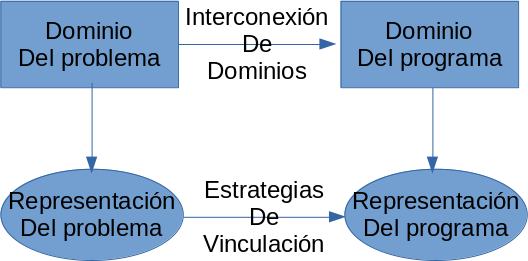
\includegraphics[width=6cm]{program_comprehension/domains.png}
    \centering
    \caption{Interrelación de Dominios}
\end{figure}

Existen diferentes estrategias\cite{BeronOliveiraCruz10} para este proceso de 
\textit{inter-relación de dominios}.
Los mismos son explicados brevemente a continuación:

\paragraph{SVS (Simultaneous Visualization Strategy)}
En esta estrategia, se utiliza información extraída dinámicamente, a través de
la instrumentación del código fuente.
Un inspector, insertado durante la instrumentación, extrae información de las funciones 
que son ejecutadas; mientras que el monitor se encarga de mostrar esta información.
De esta manera, mediante la ejecución y observación, el programador puede relacionar
el Dominio del Problema con el Dominio del Programa. 

\paragraph{BORS (Behavioral-Operational Relation Strategy)}
Al igual que la SVS, en esta estrategia también se utiliza instrumentación del código,
para extraer información del árbol de llamada de funciones.
Esta estrategia se plantea en tres pasos.
En el primero, de índole observacional, se identifican los objetos del dominio y sus interfaces,
los cuales a través de algunas técnicas son extraídos y puestos en una lista.
El segundo paso, a través de la ejecución del código ya instrumentado, construye el árbol de
llamadas.
El tercer y último paso, consiste en asociar el árbol de llamadas extraído en el segundo paso,
con el listado de interés definido en el primer paso.
Con este proceso, el programador puede relacionar y validar el comportamiento esperado del programa
con los elementos que lo ejecutan\cite{FonsecaCruzHenriquesPereira08}.

\paragraph{SVSi (Simultaneous Visualization Strategy Improved)}
Ambos enfoques anteriores presentan inconvenientes, los cuales son tratados de resolver
con esta estrategia.
SVS relaciona los dominios, pero carece de explicaciones; mientras que BORS puede proporcionarlas,
pero requiere intervención manual.
SVSi, utilizando la salida de SVS (funciones ejecutadas) como entrada para BORS, busca
suplir las falencias mencionadas.
